\documentclass[10pt]{beamer}
\usetheme{Warsaw}
\usepackage[T1]{fontenc}
\usepackage[utf8]{inputenc}
\usepackage{chronosys}
\usepackage{graphicx}
\usepackage{stmaryrd}
\usepackage{float}
\usepackage{caption}
\title{Kinetic}
\author[Demuth Axel, Geraldes Pereira Dorian]{Team member: \newline\newline Demuth Axel \newline Geraldes Pereira Dorian \newline\newline Supervisor :  \newline\newline Pierre Alliez \newline Vincent Chabannes}
\date{}
\begin{document}
\frame{\titlepage}
\begin{frame}
    \tableofcontents
\end{frame}
\section{Introduction}

\begin{frame}{Context}
\end{frame}
\begin{frame}{Objectives}
\begin{itemize}
    \item \textbf{Reading Process and Mesh Conversion: }Convert data from stl file to ply and xyz file with normals on points
    
    \item \textbf{Application of the Kinetic Algorithm}
    
    \item \textbf{Recovery of Material Labels}
    
    \item \textbf{Utilization on City Modeling}
\end{itemize}
\end{frame}
\begin{frame}{Challenges}
\begin{itemize}    
    \item \textbf{Generating point cloud from stl file}
\begin{figure}[H]
        \begin{minipage}[t]{0.25\textwidth}
            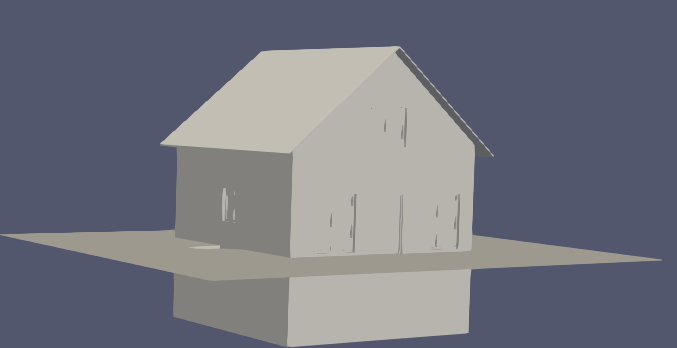
\includegraphics[width=\textwidth]{../../images/screen_kinetic/ACJasmin.png}
            \caption*{ACJasmin stl}
        \end{minipage}
        \begin{minipage}[t]{0.20\textwidth}
          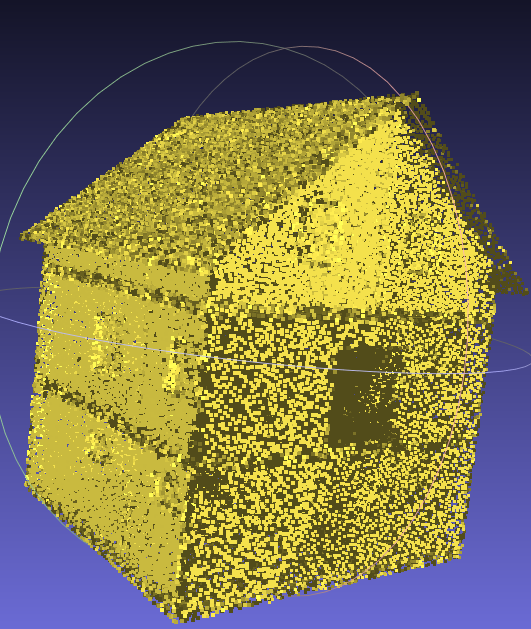
\includegraphics[width=\textwidth]{../../images/screen_kinetic/ACJasmin_point_cloud.png}
          \caption*{ACJasmin point cloud}
        \end{minipage}
\end{figure}
    \item \textbf{Parameter Optimization}
\end{itemize}
\end{frame}

\section{Tools}
\begin{frame}{Cgal}

\end{frame}
\section{Implementation}
\begin{frame}{STL}

\end{frame}
\section{Analysis of Result}
\begin{frame}{first result}

\end{frame}
\begin{frame}{last result}

\end{frame}




\begin{frame}[allowframebreaks]{reference}
    \nocite{*}
    \bibliographystyle{unsrt}
    \bibliography{../../bibliography/vfinal/report_bib}
\end{frame}

\end{document}